\documentclass[a4paper,11pt]{article}

\usepackage{latexsym}
%\usepackage[T1]{fontenc}
\usepackage[dvips]{graphicx}
\usepackage[spanish, activeacute]{babel}
\usepackage{url}
\usepackage{hyperref}
\usepackage{multicol}
\usepackage{framed}

\usepackage{practica}

%opening
\title{Trabajo Práctico 1 - \emph{Scheduling}}
\author{Sistemas Operativos - Segundo cuatrimestre de 2015}
\date{Fecha límite de entrega: 2 de Mayo de 2016, 23:59hs  GMT -03:00 }

\begin{document}
\renewcommand{\labelenumi}{\alph{enumi}$)$}
\maketitle

\section*{Parte I -- Entendiendo el simulador \texttt{simusched}}

\bigskip
\subsection*{Tareas}

Una instancia concreta de tarea (\emph{task}) se define indicando los siguientes valores:
\begin{itemize}
\item \textbf{Tipo:} de qué tipo de tarea se trata; esto determina su comportamiento general.
\item \textbf{Par'ametros:} cero o m'as n'umeros enteros que caracterizan una tarea de cierto tipo.
\item \textbf{Release time:} tiempo en que la tarea pasa al estado \emph{ready}, lista para ser ejecutada.

\end{itemize}


\subsection*{Lotes y archivos \texttt{.tsk}}

Un \emph{lote de tareas} representa una lista ordenada de tareas numeradas [0, \ldots, $n-1$] que
se especifica mediante un archivo de texto \texttt{.tsk}, de acuerdo con la siguiente sintaxis:
\begin{itemize}
        \item Las l'ineas en blanco o que comienzan con \texttt{\#} son comentarios y se ignoran.
        \item Las l'ineas de la forma ``\texttt{@\textsf{tiempo}}'', donde \textsf{tiempo} es un
        n'umero entero, indican que las tareas definidas a continuaci'on tienen un \emph{release time}
        igual a \textsf{tiempo}. Si no se agrega ninguna línea de \textsf{@tiempo}, se asume que todas las tareas empiezan en el instante cero.
        \item Las l'ineas de la forma ``\textsf{TaskName} $v_1\ v_2\ \cdots\ v_n$'', donde \textsf{TaskName}
        es un tipo de tarea y $v_1\ v_2\ \cdots\ v_n$ es una lista de cero o m'as enteros separados por espacios,
        representa una tarea de tipo \textsf{TaskName} con esos valores como par'ametro.
        \item Opcionalmente, las l'ineas del tipo anterior puede estar prefijadas por ``\texttt{*\textsf{cant}}'',
        lo cual indica que se desean \textsf{cant} copias iguales de la tarea especificada.
\end{itemize}

\subsection*{Ejemplo}

\medskip
El siguiente es un ejemplo de 4 tareas de tipo \texttt{TaskCPU} y el diagrama de Gantt asociado (para un scheduler FCFS con costo de cambio de contexto cero y un solo n'ucleo):
\begin{multicols}{4}{
\begin{framed}\noindent\scriptsize\texttt{TaskCPU 3 \\
@10: \\
TaskCPU 1 \\
@3: \\
{*}2 TaskCPU 7}
\end{framed}
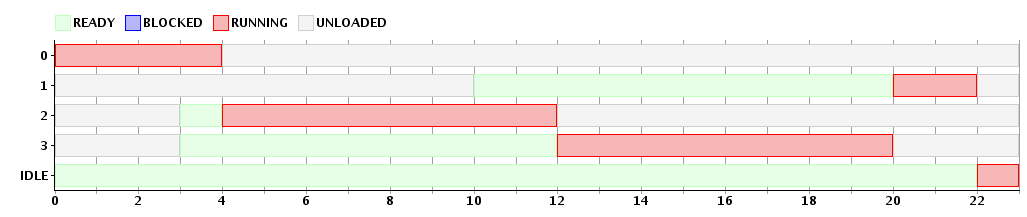
\includegraphics[keepaspectratio, width=0.72\textwidth]{ejemplo1.png}
}
\end{multicols}


\subsection*{Definici'on de tipos de tarea}

Los \emph{tipos de tarea} se definen en \texttt{tasks.cpp} y se compilan
como funciones de C++ junto con el simulador. Cada tipo de tarea est'a
representado por una 'unica funci'on que lleva su nombre y que ser'a el
cuerpo principal de la tarea a simular. Esta recibe como par'ametro
el vector de enteros que le fuera especificado en el lote, y simular'a
la utilizaci'on de recursos. Se simulan tres acciones posibles
que puede llevar a cabo una tarea, a saber:
\begin{enumerate}
        \item Utilizar el CPU durante $t$ ciclos de reloj, llamando a la funci'on \texttt{uso\_CPU($t$)}.
        \item Ejecutar una llamada bloqueante que demorar'a $t$ ciclos de
        reloj en completar, llamando a la funci'on \texttt{uso\_IO($t$)}.
        Notar que esta llamada utiliza primero el CPU durante 1 ciclo de reloj
        (para simular la ejecuci'on de la llamada bloqueante), luego de lo cual
        la tarea permanecer'a bloqueada durante $t$ ciclos de reloj.
        \item Terminar, ejecutando \texttt{return} en la funci'on. Esta acci'on
        utilizar'a un ciclo de reloj para completarse (la simulaci'on lo suma en
        concepto de ejecuci'on de una llamada \texttt{exit()}, liberaci'on de recursos, etc),
        luego del cual la tarea pasa a estado \emph{done}.
\end{enumerate}


\subsection*{Sintaxis de invocaci'on}

Para ejecutar el simulador, tras compilar con \texttt{make}, debe utilizarse la l'inea de comando:
\begin{verbatim}
    ./simusched <lote.tsk> <num_cores> <costo_cs> <costo_mi> <sched> [<params_sched>]
\end{verbatim}
\noindent donde:
\begin{itemize}
        \item \texttt{<lote.tsk>} \ es el archivo que especifica el lote de tareas a simular.
        \item \texttt{<num\_cores>} \ es la cantidad de n'ucleos de procesamiento.
        \item \texttt{<costo\_cs>} \ es el costo de cambiar de contexto.
         \item \texttt{<costo\_mi>} \ es el costo de cambiar un proceso de núcleo de procesamiento.
        \item \texttt{<sched>} \ es el nombre de la clase de scheduler a utilizar (ej. \texttt{SchedFCFS}).
        \item \texttt{<params\_sched>}  \ es una lista de cero o m'as par'ametros para el scheduler.
\end{itemize}


\subsection*{Graficaci'on de simulaciones}

Para generar un diagrama de Gantt de la simulaci'on puede utilizarse la herramienta
\texttt{graphsched.py}, que recibe por entrada estándar el formato de salida estándar
de \texttt{simusched}, y a su vez escribe por salida estándar una imagen binaria en formato PNG.

Para generar un diagrama de Gantt del uso de los cores puede utilizarse la herramienta
\texttt{graph\_cores.py}, que recibe por entrada estándar el formato de salida estándar
de \texttt{simusched}, y a su vez escribe por salida estándar una imagen binaria en formato PNG.
Requiere la biblioteca para python matplotlib (\texttt{http://matplotlib.org})


\subsection*{Ejercicios}

\begin{ejercicio}

Programar un tipo de tarea \texttt{TaskConsola}, que simular'a una tarea
interactiva. La tarea debe realizar $n$ llamadas bloqueantes, cada una de una
duraci'on al azar\footnote{\texttt{man 3 rand}} entre $bmin$ y $bmax$
(inclusive). La tarea debe recibir tres par'ametros: $n$, $bmin$ y $bmax$ (en
ese orden) que ser'an interpretados como los tres elementos del vector de
enteros que recibe la funci'on. Explique la implementación realizada y
grafique un lote que utilice el nuevo tipo de tarea.

\end{ejercicio}

\begin{ejercicio}
El grupo de de Data Mining de la facultad, reciente ganador de importante concurso internacional, est'a preparando el algoritmo para su pr'oxima victoria. Para esto necesita utilizar la 'unica m'aquina que tienen 500 ciclos de CPU.

A su vez usan la m'aquina como servidor remoto, utilizando 3 usuarios que realizan llamadas bloqueantes de 10, 20 y 30 respectivamente y de una duraci'on al azar de hasta 4 ciclos.

Escribir el lote de tareas que simule la situación del grupo. Ejecutar y graficar la simulaci'on usando el algoritmo \texttt{FCFS} para 1 y 2 y 4 núcleos con un cambio de contexto de 5 ciclos. Calcular la \emph{latencia} de cada tarea en los dos gr'aficos. Explicar qu'e desventaja tendr'ian si debe mantener este algoritmo de scheduling y s'olo tiene disponible una computadora con un n'ucleo (haga referencia a los gr'aficos y a los c'alculos anteriores para justificar su explicaci'on).
\end{ejercicio}

\begin{ejercicio}

Programar un tipo de tarea \texttt{TaskBatch} que reciba dos parámetros:
$total\_cpu$ y $cant\_bloqueos$. Una tarea de este tipo deber'a realizar
$cant\_bloqueos$ llamadas bloqueantes, en momentos elegidos
pseudoaleatoriamente. En cada tal ocasi'on, la tarea deber'a permanecer
bloqueada durante exactamente dos (4) ciclos de reloj. El tiempo de CPU total
que utilice una tarea \texttt{TaskBatch} deber'a ser de $total\_cpu$ ciclos de
reloj (incluyendo el tiempo utilizado para lanzar las llamadas bloqueantes; no
as'i el tiempo en que la tarea permanezca bloqueada). Explique la
implementación realizada y grafique un lote que utilice 4 tareas \texttt{TaskBatch}
con parámetros diferentes y que corra con el scheduler \texttt{FCFS}.

\end{ejercicio}


%\newpage
\section*{Parte II: Extendiendo el simulador con nuevos \emph{schedulers}}

Un algoritmo de \emph{scheduling} se implementa mediante una clase de C++
(una nueva subclase que herede de \texttt{SchedBase}). A continuaci'on se
describe la API correspondiente.

Para ser un \emph{scheduler} v'alido, una tal clase debe implementar al
menos tres m'etodos: \texttt{load(pid)}, \texttt{unblock(pid)} y \texttt{tick(cpu, motivo)}.

Cuando una tarea nueva llega al sistema el simulador ejecutar'a el m'etodo
\texttt{void load(pid)} del scheduler para notificar al mismo de la llegada
de un nuevo \texttt{pid}. Se garantiza que en las sucesivas llamadas a \texttt{load}
el valor de \texttt{pid} comenzar'a en 0 e ir'a aumentando de a 1.

Por cada \emph{tick} del reloj de la m'aquina el simulador ejecutar'a
el m'etodo \texttt{int tick(cpu, motivo)} del scheduler. El parámetro \texttt{cpu} indica qu'e CPU es el que realiza el tick. El par'ametro
\texttt{motivo} indica qu'e ocurri'o con la tarea que estuvo en posesi'on
del CPU durante el 'ultimo ciclo de reloj:
\begin{itemize}
        \item \texttt{TICK}: la tarea consumi'o todo el ciclo utilizando el CPU.
        % \vspace{-3mm}
        \item \texttt{BLOCK}: la tarea ejecut'o una llamada
        bloqueante o permaneci'o bloqueada durante el 'ultimo ciclo.
        % \vspace{-3mm}
        \item \texttt{EXIT}: la tarea termin'o (ejecut'o \texttt{return}).
\end{itemize}

El m'etodo \texttt{tick()} del scheduler debe tomar una decisi'on y luego
devolver el \texttt{pid} de la tarea elegida para ocupar el pr'oximo ciclo
de reloj (o, en su defecto, la constante \texttt{IDLE\_TASK}).
El scheduler dispone de la funci'on \texttt{current\_pid()} para saber
qu'e proceso est'a usando el CPU.

\medskip
Por 'ultimo, en el caso que una tarea se haya bloqueado, el simulador llamar'a al m'etodo
\texttt{void unblock(pid)} del scheduler cuando la tarea \texttt{pid} deje de estar bloqueada.
En la siguiente llamada a \texttt{tick} este \texttt{pid} estar'a disponible
para ejecutar.

\subsection*{Ejercicios}

\begin{ejercicio}
Completar la implementaci'on del scheduler \emph{Round-Robin} implementando
los m'etodos de la clase \texttt{SchedRR} en los archivos
\texttt{sched\_rr.cpp} y \texttt{sched\_rr.h}. La implementaci'on recibe como primer par'ametro
la cantidad de n'ucleos y a continuación los valores de sus respectivos \emph{quantums}. Debe utilizar una única cola global, permitiendo así la migración de procesos entre núcleos.
\end{ejercicio}

\begin{ejercicio}
Diseñe un lote con 3 tareas de tipo \texttt{TaskCPU} de 70 ciclos y 2 de tipo  \texttt{TaskConsola} con 3 llamadas bloqueantes de 3 ciclos de duración cada una. Ejecutar y graficar la simulaci'on utilizando el scheduler \emph{Round-Robin} con quantum 2, 10 y 50.

Con un cambio de contexto de 2 ciclos y un sólo núcleo calcular la \emph{latencia}, el \emph{waiting time} y el tiempo total de ejecuci'on de las cinco tareas para cada quantum. ¿En cu'al es mejor cada uno? ¿Por qu'e ocurre esto?
\end{ejercicio}


\begin{ejercicio}
Grafique el mismo lote de tareas del ejercicio anterior para el scheduler \emph{FCFS}. Haciendo referencia a lo que se observa en los gr'aficos de este ejercicio y el anterior, explique las diferencias entre un scheduler \emph{Round-Robin} y un \emph{FCFS}.
\end{ejercicio}

% \begin{ejercicio}
% Completar la implementaci'on del scheduler \emph{Multilevel Feedback Queue} implementando
% los m'etodos de la clase \texttt{SchedMFQ} en los archivos
% \texttt{sched\_mfq.cpp} y \texttt{sched\_mfq.h}. La implementaci'on
% debe utilizar $n$ colas con \emph{Round-Robin} en cada una con los par'ametros
% que se detallan a continuaci'on.
% \begin{itemize}
%       \item Las $n$ colas se numeran de 0 a $n-1$ siendo 0 la de mayor prioridad.
%       \vspace{-3mm}
%       \item El constructor recibe como par'ametro $n$ n'umeros $q_i$ indicando el \emph{quantum} de la cola $i$.
%       \vspace{-3mm}
%       \item Al iniciar una tarea comienza al final de la cola de mayor prioridad.
%       \vspace{-3mm}
%       \item Siempre se ejecuta la primer tarea de la cola no vac'ia de mayor prioridad. Si esta tarea
%       consume todo su \emph{quantum} sin bloquearse entonces pasa al final de la cola inmediatamente de inferior prioridad (si hay).
%       Si esta tarea se bloquea antes de agotar su \emph{quantum}, entonces (cuando se desbloquee)
%       se reencola al final de la cola inmediatamente de superior prioridad (si hay).
%       \vspace{-3mm}
%       \item Si todas las colas est'an vac'ias se ejecuta \texttt{IDLE\_TASK}.
% \end{itemize}
% \end{ejercicio}



%\newpage

\begin{ejercicio}
El scheduler \emph{SchedMistery} fue creado por docentes investigadores de nuestra materia y ha sido destacado en la última publicación de \texttt{ACM - SIGOPS}, \texttt{Operating Systems Review}. Desde entonces, numerosos investigadores de todo el mundo nos han contactado para pedirnos su c'odigo fuente. Sin embargo, su c'odigo no aparece en ninguno de los repositorios de la materia y nadie parece recordar qui'enes hab'ian estado detr'as de su implementaci'on.

Se les pide experimentar con dicho scheduler (aprovechando que hemos conseguido el c'odigo objeto) y replicar su funcionamiento en \emph{SchedNoMistery}. Graficar como máximo tres lotes de tareas utilizados en los experiementos y explicar en cada uno por separado qué características de SchedMistery identificaron con ese lote. Nota: El scheduler \textbf{funciona para un solo core} y toma uno o más argumentos numericos.
\end{ejercicio}

\begin{ejercicio}
Implemente un scheduler \emph{Round-Robin} que no permita la migración de procesos entre núcleos (\texttt{SchedRR2}). La asignación de CPU se debe realizar en el momento en que se produce la carga de un proceso (\texttt{load}). El núcleo correspondiente a un nuevo proceso será aquel con menor cantidad de procesos activos totales (RUNNING + BLOCKED + READY). Explique un escenario real donde la migraci'on de n'ucleos sea beneficiosa y uno donde no (mencione especificamente qu'e m'etricas de comparaci'on vistas en la materia mejorar'ian en cada caso). Diseñe un lote de tareas en nuestro simulador que represente a cada uno de esos escenarios y grafique su resultado para cada implementaci'on. Calcule y compare en cada gr'afico las m'etrica que mencion'o.
\end{ejercicio}

\bigskip

\section*{Informe}

El informe \textbf{DEBE} contener las siguiente secciónes:

\begin{itemize}
    \item Carátula (1 carilla)

    \item Índice (1 carrilla)

    \item \textbf{1 sección} por ejercicio
\end{itemize}

El informe \textbf{NO DEBE} superar las 20 carillas.

\section*{Código}

\textbf{DEBEN} modificar el Makefile entregado para que soporte los siguientes
\textit{targets}

\begin{itemize}
    \item \texttt{make ejercicio1}

    \item $\cdots$

    \item \texttt{make ejercicio8}
\end{itemize}

Donde cada \textit{target} \textbf{DEBE} generar los gráficos presentados en
el informe para el ejercicio indicado.

El código \textbf{DEBE} estar comentado.

\section*{Entrega}

El tiempo \textbf{LÍMITE} de entrega del trabajo es el lunes 2 de
mayo a las 23:59 GMT -3.\\

La entrega se realizará por correo electrónico a la dirección
\textbf{sisopdc@gmail.com} cuyo asunto \textbf{DEBE} decir:

\begin{center}
    \textbf{[TP1] Entrega TP1}
\end{center}

y cuyo cuerpo \textbf{DEBE} contener los datos de cada integrante:

\begin{center}
    \textbf{$Apellido_1$, $Nombre_1$, $LU_1$, $Correo$ $Electr\acute{o}nico_1$}\\
    \textbf{$Apellido_2$, $Nombre_2$, $LU_2$, $Correo$ $Electr\acute{o}nico_2$}\\
    \textbf{$Apellido_3$, $Nombre_3$, $LU_3$, $Correo$ $Electr\acute{o}nico_3$}\\
\end{center}

En la entrega \textbf{DEBERÁN} adjuntar únicamente:

\begin{itemize}
    \item El documento del informe (en \textbf{PDF}).

    \item El código fuente \textbf{completo junto con el Makefile modificado}.
\end{itemize}

\textbf{NO} incluir código compilado.

\end{document}

\end{document}
